\documentclass{article}

% if you need to pass options to natbib, use, e.g.:
%     \PassOptionsToPackage{numbers, compress}{natbib}
% before loading neurips_2026

% The authors should use one of these tracks.
% Before accepting by the NeurIPS conference, select one of the options below.
% 0. "default" for submission
% \usepackage{neurips_2026}
% the "default" option is equal to the "main" option, which is used for the Main Track with double-blind reviewing.
% 1. "main" option is used for the Main Track
%  \usepackage[main]{neurips_2026}
% 2. "position" option is used for the Position Paper Track
%  \usepackage[position]{neurips_2026}
% 3. "eandd" option is used for the Evaluations & Datasets Track
 % \usepackage[eandd]{neurips_2026}
% 4. "creativeai" option is used for the Creative AI Track
%  \usepackage[creativeai]{neurips_2026}
% 5. "sglblindworkshop" option is used for the Workshop with single-blind reviewing
 % \usepackage[sglblindworkshop]{neurips_2026}
% 6. "dblblindworkshop" option is used for the Workshop with double-blind reviewing
%  \usepackage[dblblindworkshop]{neurips_2026}
% 7. "education" option is used for the Education Track
%  \usepackage[education]{neurips_2026}


% After being accepted, the authors should add "final" behind the track to compile a camera-ready version.
% 1. Main Track
 % \usepackage[main, final]{neurips_2026}
% 2. Position Paper Track
%  \usepackage[position, final]{neurips_2026}
% 3. Evaluations & Datasets Track
 % \usepackage[eandd, final]{neurips_2026}
% 4. Creative AI Track
%  \usepackage[creativeai, final]{neurips_2026}
% 5. Workshop with single-blind reviewing
%  \usepackage[sglblindworkshop, final]{neurips_2026}
% 6. Workshop with double-blind reviewing
%  \usepackage[dblblindworkshop, final]{neurips_2026}
% Note. For the workshop paper template, both \title{} and \workshoptitle{} are required, with the former indicating the paper title shown in the title and the latter indicating the workshop title displayed in the footnote.
% For workshops (5., 6.), the authors should add the name of the workshop, "\workshoptitle" command is used to set the workshop title.
% \workshoptitle{WORKSHOP TITLE}
% 7. Education Track
% \usepackage[education, final]{neurips_2026}

% Use final mode for the course report so the rendered PDF does not show
% the preprint footer text.
\usepackage[main, final]{neurips_2026}

% to avoid loading the natbib package, add option nonatbib:
%    \usepackage[nonatbib]{neurips_2026}

\usepackage[utf8]{inputenc} % allow utf-8 input
\usepackage[T1]{fontenc}    % use 8-bit T1 fonts
\usepackage{hyperref}       % hyperlinks
\usepackage{url}            % simple URL typesetting
\usepackage{booktabs}       % professional-quality tables
\usepackage{amsfonts}       % blackboard math symbols
\usepackage{amsmath}
\usepackage{nicefrac}       % compact symbols for 1/2, etc.
\usepackage{microtype}      % microtypography
\usepackage{xcolor}         % colors
\usepackage{graphicx}
\hypersetup{hidelinks}
\makeatletter
\renewcommand{\@noticestring}{}
\makeatother

% Note. For the workshop paper template, both \title{} and \workshoptitle{} are required, with the former indicating the paper title shown in the title and the latter indicating the workshop title displayed in the footnote. 
\title{Report for Project 5: Image Captioning with a CNN--LSTM Encoder--Decoder\\
       on the Flickr8k Dataset}


% The \author macro works with any number of authors. There are two commands
% used to separate the names and addresses of multiple authors: \And and \AND.
%
% Using \And between authors leaves it to LaTeX to determine where to break the
% lines. Using \AND forces a line break at that point. So, if LaTeX puts 3 of 4
% authors names on the first line, and the last on the second line, try using
% \AND instead of \And before the third author name.


\author{
  Reza Naziri\\
  \texttt{e12322888@student.tuwien.ac.at} \\
  \And
  Alireza Niroumand \\
  \texttt{e12127666@student.tuwien.ac.at} \\
  \And
  Emanuel Klatzer \\
  \texttt{e12020639@student.tuwien.ac.at} \\
}


\begin{document}


\maketitle


\begin{abstract}
Image captioning requires a model to both understand the visual content of an
image and express that understanding as a fluent natural-language sentence. In
this project we implement, train and evaluate a complete image captioning system
based on the classical encoder--decoder paradigm of \emph{Show and Tell}
\citep{vinyals2015show}. A ResNet-50 convolutional encoder, pretrained on
ImageNet and used with a frozen backbone, compresses each image into a single
256-dimensional feature vector; an LSTM decoder then generates the caption one
word at a time, conditioned on that vector. The system is trained on Flickr8k
(8{,}091 images, 40{,}455 captions) with teacher forcing and a cross-entropy
objective that ignores padding positions, and evaluated with corpus BLEU-1
through BLEU-4 against five human reference captions per image. Our model
achieves a BLEU-1 of \textbf{0.580} and a BLEU-4 of \textbf{0.172} on a
held-out test split constructed \emph{by image} to eliminate data leakage. We
present a qualitative analysis of success and failure cases, and a discussion
connecting each observed weakness to a concrete architectural cause: rare words
lost to the vocabulary frequency threshold, genericness induced by greedy
decoding, and spatial detail lost to the single-vector image bottleneck in the
absence of an attention mechanism. The full pipeline is implemented as a
modular, seeded and unit-tested Python package (49 tests) to ensure
reproducibility.
\end{abstract}


% ===============================================================================
\section{Introduction and motivation}

Image captioning is the task of automatically producing a natural-language description of an image.
Unlike image classification, which assigns a single label from a fixed set, captioning requires a model to recognise the objects present, infer their attributes, actions and mutual relationships, 
and then compose all of this into a grammatically well-formed and semantically relevant sentence.
It therefore sits precisely at the intersection of computer vision and natural language processing,
and serves as a natural benchmark for whether a system's visual representation is rich enough to be 
\emph{verbalised} rather than merely classified.

The task has direct practical value. Automatically generated alt-text makes images accessible to visually impaired users; caption-level annotations enable semantic search and indexing of large
image collections; and in robotics, describing a scene in language is a prerequisite for grounded human--robot communication.

The dominant formulation, popularised by \citet{vinyals2015show} and developed in parallel by related work such as \citet{karpathy2015deep}, treats captioning as a translation-like problem: a convolutional neural network \emph{encodes} the image into a fixed-length vector, and a recurrent neural network \emph{decodes} that vector into a word sequence. This is the architecture we implement.

Our contributions in this project are:
\begin{itemize}
  \item A complete PyTorch implementation of a CNN--LSTM captioning model with a
        pretrained, frozen ResNet-50 encoder and an LSTM decoder trained with
        teacher forcing.
  \item A leakage-free evaluation protocol in which the train/validation/test
        split is performed over \emph{unique images} rather than caption rows.
  \item A corpus-level BLEU-1..4 evaluation against five human references per
        image, complemented by a qualitative analysis of success and failure cases.
  \item A modular, deterministically seeded and unit-tested codebase (49 tests)
        that runs identically on a laptop, Google Colab or Kaggle.
\end{itemize}


% ===============================================================================
\section{Technical background and preliminaries}

\subsection{Convolutional neural networks and transfer learning}

Convolutional neural networks (CNNs) learn a hierarchy of visual features through stacked convolution, normalisation and non-linear activation layers. ResNet-50 \citep{he2016deep} is a 
50-layer residual network whose skip connections allow gradients to propagate through very deep 
stacks, mitigating the vanishing-gradient problem. Pretrained on ImageNet \citep{deng2009imagenet},
its learned features --- edges, textures, object parts --- transfer well to downstream vision tasks.

\emph{Transfer learning} exploits this: rather than training from random initialisation, we reuse the pretrained weights. In the extreme case the backbone is \emph{frozen}, i.e.\ its parameters receive no gradient updates and it acts purely as a fixed feature extractor. Only a small task-specific head is learned.

\subsection{Recurrent sequence modelling with LSTMs}

A recurrent neural network processes a sequence one token at a time, maintaining a hidden state that summarises everything seen so far. The Long Short-Term Memory (LSTM) cell \citep{hochreiter1997long} augments this with a gated memory cell, allowing the network to retain information over longer spans than a vanilla RNN.

\subsection{The encoder--decoder formulation}

Let $I$ be an image and $Y = (y_1, \dots, y_T)$ its caption. The model factorises the conditional probability of the caption autoregressively:
\begin{equation}
  P(Y \mid I; \theta) = \prod_{t=1}^{T} P\!\left(y_t \mid y_{<t},\, I;\, \theta\right),
\end{equation}
where $\theta$ are the trainable parameters. Training minimises the negative log-likelihood of the ground-truth captions, i.e.\ a token-level cross-entropy loss. The key idea of \emph{Show and Tell} \citep{vinyals2015show} is to inject the image by treating the encoder's feature vector as the \emph{first token} of the sequence.

\subsection{Teacher forcing}

During training the decoder is fed the \emph{ground-truth} previous word rather than its own previous prediction. This stabilises and accelerates training. At inference time the model must consume its own outputs --- a train/test mismatch known as exposure bias.

\subsection{Evaluation metric: BLEU}

BLEU (Bilingual Evaluation Understudy) \citep{papineni2002bleu} measures
$n$-gram overlap between a candidate sentence and one or more references.
BLEU-$n$ computes a modified precision over $n$-grams and combines it with a
brevity penalty that discourages short outputs. Because BLEU-4 requires four
consecutive words to match, it is strictly harder than BLEU-1. We report
\emph{corpus} BLEU with NLTK smoothing (\texttt{SmoothingFunction.method1}).

\subsection{Dataset: Flickr8k}

We use the Flickr8k dataset \citep{hodosh2013framing}, obtained via \texttt{kagglehub} (\texttt{adityajn105/flickr8k}, approximately 1\,GB). Flickr8k was chosen over MS-COCO \citep{lin2014microsoft} because it is small enough to train on a free-tier GPU within the project's compute budget. Table~\ref{tab:dataset} summarises its properties.

\begin{table}[h]
  \caption{Flickr8k dataset statistics, verified programmatically.}
  \label{tab:dataset}
  \centering
  \begin{tabular}{lr}
    \toprule
    Property & Value \\
    \midrule
    Images & 8{,}091 \\
    Captions & 40{,}455 \\
    Captions per image (min / max / mean) & 5 / 5 / 5.0 \\
    Missing or unused images & 0 \\
    \bottomrule
  \end{tabular}
\end{table}

\subsection{Image preprocessing}

Each image is: (i) resized so that its shorter side is 256 pixels; (ii) centre-cropped to $224 \times 224$; (iii) converted to a float tensor; and (iv) normalised with the ImageNet mean $(0.485, 0.456, 0.406)$ and standard deviation
$(0.229, 0.224, 0.225)$.

\subsection{Caption preprocessing and vocabulary}

Captions are lowercased and tokenised with \verb|\w+|, which extracts contiguous word-character sequences and removes punctuation. Four special tokens occupy fixed indices: \texttt{<pad>}$=0$, \texttt{<start>}$=1$, \texttt{<end>}$=2$, \texttt{<unk>}$=3$. Words appearing fewer than
$\tau_{\text{freq}} = 5$ times map to \texttt{<unk>}; the resulting vocabulary
contains 2{,}982 entries. The vocabulary is built in sorted order for
determinism.

\subsection{Splitting by image}

We split over \emph{unique image names} (not caption rows) with seed 42: 80\,/\,10\,/\,10 into train, validation and test. All five captions of an image stay in the same split, preventing data leakage.

% ===============================================================================
\section{Methodology}

\subsection{Model architecture}

\subsubsection{Encoder: frozen ResNet-50}

A ResNet-50 with ImageNet weights has its final classification layer removed. The backbone maps $I \in \mathbb{R}^{3 \times 224 \times 224}$ to a 2048-dimensional vector $\mathbf{f}$ after global average pooling. A trainable projection and batch normalisation produce the image embedding:
\begin{equation}
  \mathbf{v} = \mathrm{BN}\!\left( \mathbf{W}_{\text{proj}} \mathbf{f} +
  \mathbf{b}_{\text{proj}} \right), \qquad
  \mathbf{W}_{\text{proj}} \in \mathbb{R}^{256 \times 2048}.
\end{equation}
The backbone is \textbf{frozen}: $\approx$\textbf{4.4M trainable} vs $\approx$\textbf{23.5M frozen} parameters.

\subsubsection{Decoder: LSTM language model}

The decoder has: an embedding layer ($|V| \to 256$) with dropout $p=0.5$; a single LSTM layer (hidden size 512); and a linear layer ($512 \to |V|$).

\subsubsection{Training alignment}

For caption $(\texttt{<start>}, w_1, \dots, w_K, \texttt{<end>})$ of length $T$:
\begin{align*}
  \text{input}  &= \big(\mathbf{v},\, \mathbf{e}_{\texttt{<start>}},\,
                    \mathbf{e}_{w_1},\, \dots,\, \mathbf{e}_{w_K}\big), \\
  \text{target} &= \big(\texttt{<start>},\, w_1,\, \dots,\, w_K,\,
                    \texttt{<end>}\big).
\end{align*}

\subsubsection{Inference: greedy decoding}

At inference the model initialises from the image vector and greedily selects the highest-scoring word at each step, feeding it back until \texttt{<end>} or maximum length is reached.

\subsection{Training setup}

\subsubsection{Objective and optimisation}

Cross-entropy loss with \texttt{ignore\_index=0} (\texttt{<pad>}):
\begin{equation}
  \mathcal{L} = - \frac{1}{N} \sum_{i=1}^{B} \sum_{t=1}^{T}
  \mathbb{1}\!\left[ y^{(i)}_t \neq \texttt{<pad>} \right]
  \log P\!\left( y^{(i)}_t \mid y^{(i)}_{<t}, I^{(i)} \right).
\end{equation}
Adam \citep{kingma2014adam} with $\text{lr} = 3 \times 10^{-4}$ on trainable
parameters only. Full hyperparameters are in Table~\ref{tab:hyperparams}.

\begin{table}[h]
  \caption{Model and training hyperparameters.}
  \label{tab:hyperparams}
  \centering
  \begin{tabular}{ll}
    \toprule
    Hyperparameter & Value \\
    \midrule
    CNN backbone         & ResNet-50 (ImageNet pretrained, frozen) \\
    Embedding size       & 256 \\
    LSTM hidden size     & 512 \\
    LSTM layers          & 1 \\
    Dropout              & 0.5 \\
    Vocabulary size      & 2{,}982 (threshold $\tau=5$) \\
    Max caption length   & 50 tokens \\
    \midrule
    Loss                 & Cross-entropy, \texttt{ignore\_index=<pad>} \\
    Optimiser            & Adam, lr $= 3\times10^{-4}$ \\
    Batch size           & 64 \\
    Epochs               & 20 \\
    Train / Val / Test   & 80 / 10 / 10, split by image \\
    Random seed          & 42 \\
    Trainable params     & $\approx 4.4$M \\
    Frozen params        & $\approx 23.5$M \\
    \bottomrule
  \end{tabular}
\end{table}

\subsubsection{Reproducibility and software engineering}

The pipeline is split into eight importable modules:
\texttt{config}, \texttt{vocabulary}, \texttt{dataset}, \texttt{encoder},
\texttt{decoder}, \texttt{model}, \texttt{train}, \texttt{evaluate}.
We wrote 49 unit tests (\texttt{pytest}) covering vocabulary behaviour, dataset
shapes and split disjointness, encoder/decoder forward passes, and BLEU
correctness. All tests use synthetic data and run in under a minute.

% ===============================================================================
\section{Experiments and results}

\subsection{Training dynamics}

Figure~\ref{fig:loss} shows the training and validation loss over 20 epochs.
The training loss decreases from \textbf{4.1753} at epoch~1 to \textbf{1.8919}
at epoch~20. The validation loss reaches its minimum of \textbf{2.6014} at
epoch~\textbf{15}, after which it plateaus. The checkpoint from that epoch is
used for all results below.

\begin{figure}[h]
  \centering
  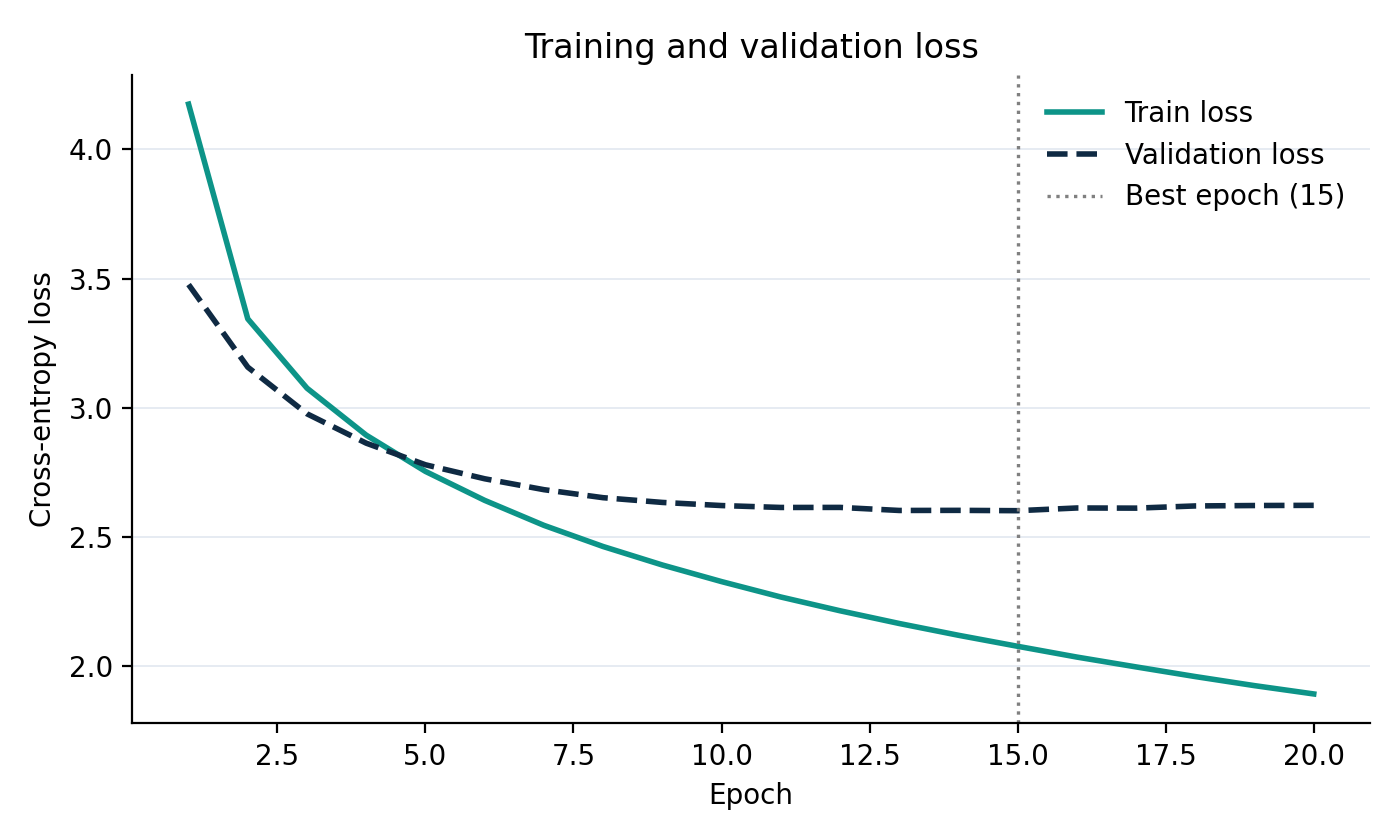
\includegraphics[width=0.72\textwidth]{loss_curve.png}
  \caption{Training and validation cross-entropy loss over 20 epochs. The dotted
           vertical line marks epoch~15, the best validation checkpoint.}
  \label{fig:loss}
\end{figure}

\subsection{Quantitative results}

Table~\ref{tab:bleu} reports corpus BLEU on the held-out test split.

\begin{table}[h]
  \caption{Corpus BLEU scores on the Flickr8k test split (810 images, five
           references each). Literature values are for context only --- they use
           different splits and (for \citet{xu2015show}) attention.}
  \label{tab:bleu}
  \centering
  \begin{tabular}{lcccc}
    \toprule
    Model & BLEU-1 & BLEU-2 & BLEU-3 & BLEU-4 \\
    \midrule
    \textbf{Ours} (frozen ResNet-50 + LSTM, greedy)
      & \textbf{0.580} & \textbf{0.395} & \textbf{0.261} & \textbf{0.172} \\
    \midrule
    Show and Tell / Google NIC, as reported by \citet{xu2015show} & 0.63 & 0.41 & 0.27 & --- \\
    Soft attention \citep{xu2015show}     & 0.67 & 0.448 & 0.299 & 0.195 \\
    \bottomrule
  \end{tabular}
\end{table}

\subsection{Qualitative results}

\paragraph{Successes:}
The model reliably identifies the main subject and action in canonical scenes
--- people playing, animals running, outdoor activities --- producing
grammatically well-formed and semantically relevant captions. On clear,
unambiguous images the generated caption closely matches the vocabulary and
structure of the human references.

\paragraph{Failures:}
Failure cases are systematic. First, unusual objects whose words appear fewer
than five times in Flickr8k are absent from the vocabulary and map to
\texttt{<unk>}, forcing the model to fall back on a generic substitute. Second,
without an attention mechanism the entire image is compressed into a single
256-dimensional vector; small or off-centre objects are frequently lost. Third,
greedy decoding biases captions towards high-frequency, low-information phrases.

Figure~\ref{fig:qualitative} illustrates these patterns: the model captures
salient dog-related scenes in some cases, but also produces fluent yet visually
incorrect captions when the scene requires finer visual grounding.

\begin{figure}[t]
  \centering
  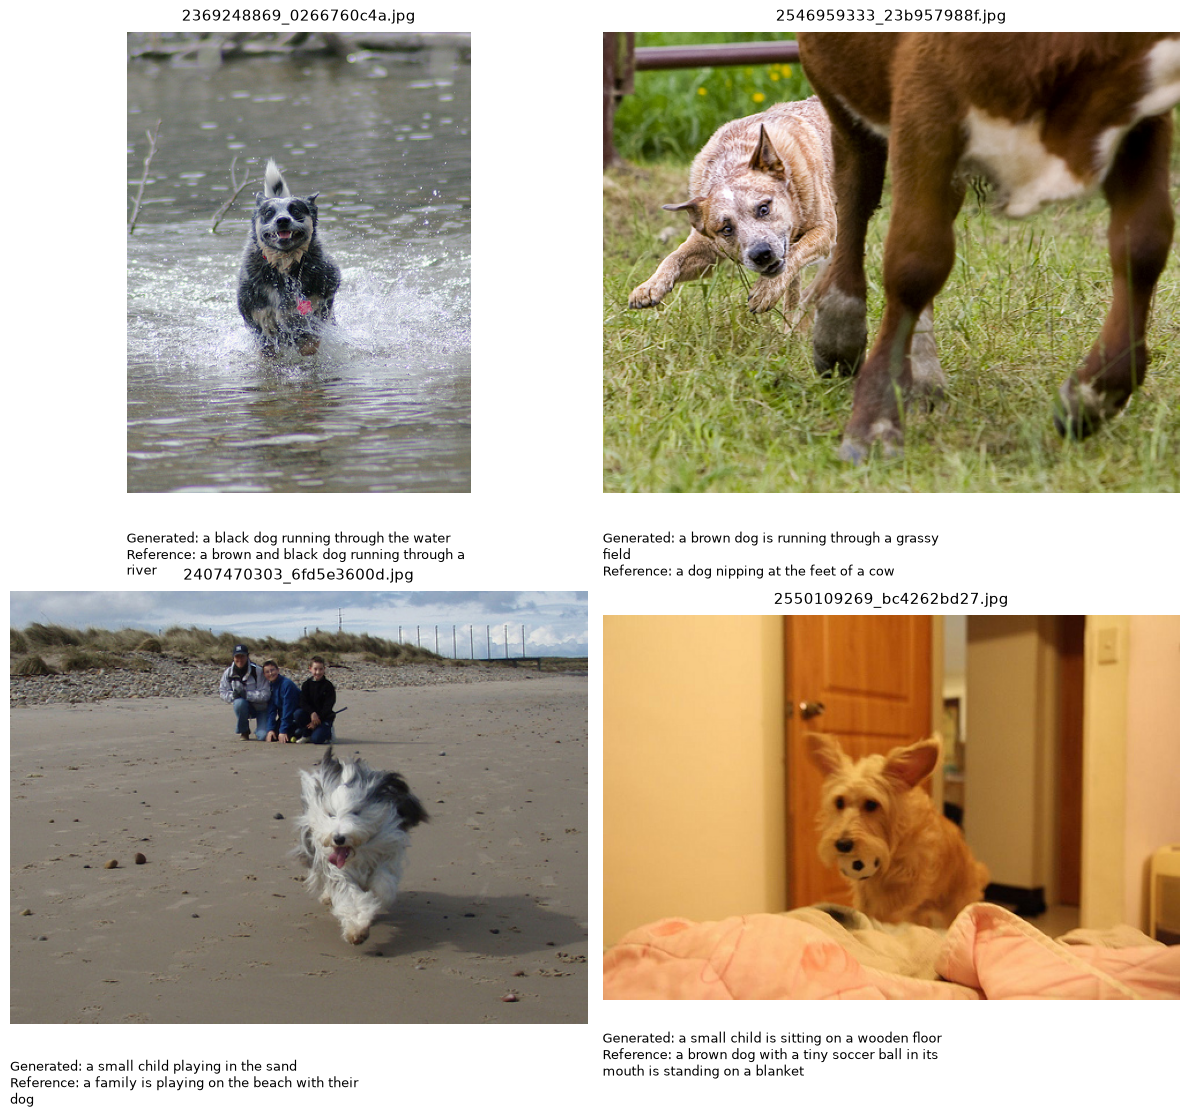
\includegraphics[width=\textwidth]{qualitative_eval.png}
  \caption{Generated captions and reference captions for four test images.
  The top-left example shows a close semantic match between prediction and
  reference. The remaining examples highlight common limitations of the model:
  confusion between visually or contextually related concepts, loss of small or
  off-centre details, and a bias towards high-frequency caption patterns such as
  ``a small child''.}
  \label{fig:qualitative}
\end{figure}

\subsection{Discussion}

\subsubsection{What works}

The model produces fluent and broadly relevant captions for common scenes.
Freezing the backbone makes training fast and stable: only $\approx 16\%$ of
parameters receive gradients, which acts as a strong regulariser on 6{,}500
training images.

\subsubsection{Where it struggles, and why}

Each observed weakness traces to a specific design decision.

\paragraph{Rare objects become \texttt{<unk>}:}
The frequency threshold $\tau=5$ structurally prevents the model from naming
rare objects. Lowering the threshold would expand the vocabulary but give too
few training examples per word.

\paragraph{Greedy decoding yields generic captions:}
Committing irrevocably to the highest-scoring word at each step biases the model
towards safe, common phrases. Beam search directly targets this.

\paragraph{Frozen backbone limits visual adaptation:}
The encoder's features are fixed to what was useful for ImageNet. Fine-grained
distinctions not needed for classification cannot be recovered by decoder
training alone.

\paragraph{No attention creates an information bottleneck:}
Compressing the entire image into one 256-dim vector loses small or off-centre
details. An attention mechanism \citep{xu2015show} would let the decoder
re-weight a spatial grid of features at each generation step.

\subsubsection{Limitations of the evaluation}

BLEU penalises correct captions that use different wording. Metrics such as
CIDEr \citep{vedantam2015cider} and METEOR would give a more faithful picture.
Results are from a single run; averaging over seeds would yield more robust
claims.


% ===============================================================================
\section{Conclusion and future work}

We implemented, trained and evaluated a complete CNN--LSTM image captioning
system on Flickr8k. The system achieves a BLEU-1 of \textbf{0.580} and a
BLEU-4 of \textbf{0.172}, producing fluent captions for common scenes while
remaining generic on unusual ones. The most impactful next steps are:
\begin{itemize}
  \item \textbf{Attention} \citep{xu2015show} to remove the single-vector bottleneck.
  \item \textbf{Beam search} to improve decoding quality without retraining.
  \item \textbf{Backbone fine-tuning} to adapt visual features to Flickr8k.
  \item \textbf{Larger dataset} (MS-COCO \citep{lin2014microsoft}) for a wider vocabulary.
\end{itemize}

% ===============================================================================
\section{Division of work}

\textbf{Emanuel Klatzer} set up the project repository and dependency
management, implemented the dataset download and integrity verification, designed
and validated the ResNet-compatible image preprocessing pipeline, and drafted the
introduction and dataset sections of this report.

\textbf{Reza Naziri} implemented the caption tokenisation and vocabulary, the
PyTorch \texttt{Dataset}, collate function and leakage-free split, the CNN
encoder, the LSTM decoder and the combined \texttt{CaptioningModel}, together
with the accompanying unit tests, and wrote the methodology and training-setup
sections.

\textbf{Alireza Niroumand} implemented the training loop with validation and
checkpointing, the BLEU evaluation pipeline and the qualitative visualisation
scripts, ran the training experiments, and wrote the results and discussion
sections.

All three members jointly designed the architecture, reviewed each other's code,
and prepared the presentation. The 49-test \texttt{pytest} suite was a shared
effort.

\medskip\noindent
Source code: \url{https://github.com/reza-nz/image-captioning-project}

\newpage

\bibliographystyle{plainnat}
\begin{thebibliography}{90}

\bibitem[Deng et al.(2009)]{deng2009imagenet}
J.~Deng, W.~Dong, R.~Socher, L.-J. Li, K.~Li, and L.~Fei-Fei.
\newblock {ImageNet}: A large-scale hierarchical image database.
\newblock In \emph{CVPR}, pages 248--255, 2009.
\newblock \url{https://doi.org/10.1109/CVPR.2009.5206848}

\bibitem[He et al.(2016)]{he2016deep}
K.~He, X.~Zhang, S.~Ren, and J.~Sun.
\newblock Deep residual learning for image recognition.
\newblock In \emph{CVPR}, pages 770--778, 2016.
\newblock \url{https://doi.org/10.1109/CVPR.2016.90}

\bibitem[Hodosh et al.(2013)]{hodosh2013framing}
M.~Hodosh, P.~Young, and J.~Hockenmaier.
\newblock Framing image description as a ranking task: Data, models and evaluation metrics.
\newblock \emph{Journal of Artificial Intelligence Research}, 47:853--899, 2013.
\newblock \url{https://doi.org/10.1613/jair.3994}

\bibitem[Hochreiter and Schmidhuber(1997)]{hochreiter1997long}
S.~Hochreiter and J.~Schmidhuber.
\newblock Long short-term memory.
\newblock \emph{Neural Computation}, 9(8):1735--1780, 1997.
\newblock \url{https://doi.org/10.1162/neco.1997.9.8.1735}

\bibitem[Karpathy and Fei-Fei(2015)]{karpathy2015deep}
A.~Karpathy and L.~Fei-Fei.
\newblock Deep visual-semantic alignments for generating image descriptions.
\newblock In \emph{CVPR}, pages 3128--3137, 2015.
\newblock \url{https://doi.org/10.1109/CVPR.2015.7298932}

\bibitem[Kingma and Ba(2015)]{kingma2014adam}
D.~P. Kingma and J.~Ba.
\newblock Adam: A method for stochastic optimization.
\newblock In \emph{ICLR}, 2015.
\newblock \url{https://doi.org/10.48550/arXiv.1412.6980}

\bibitem[Lin et al.(2014)]{lin2014microsoft}
T.-Y. Lin et al.
\newblock {Microsoft COCO}: Common objects in context.
\newblock In \emph{ECCV}, pages 740--755, 2014.
\newblock \url{https://doi.org/10.1007/978-3-319-10602-1_48}

\bibitem[Papineni et al.(2002)]{papineni2002bleu}
K.~Papineni, S.~Roukos, T.~Ward, and W.-J. Zhu.
\newblock {BLEU}: A method for automatic evaluation of machine translation.
\newblock In \emph{ACL}, pages 311--318, 2002.
\newblock \url{https://doi.org/10.3115/1073083.1073135}

\bibitem[Vedantam et al.(2015)]{vedantam2015cider}
R.~Vedantam, C.~L. Zitnick, and D.~Parikh.
\newblock {CIDEr}: Consensus-based image description evaluation.
\newblock In \emph{CVPR}, pages 4566--4575, 2015.
\newblock \url{https://doi.org/10.1109/CVPR.2015.7299087}

\bibitem[Vinyals et al.(2015)]{vinyals2015show}
O.~Vinyals, A.~Toshev, S.~Bengio, and D.~Erhan.
\newblock Show and tell: A neural image caption generator.
\newblock In \emph{CVPR}, pages 3156--3164, 2015.
\newblock \url{https://doi.org/10.1109/CVPR.2015.7298935}

\bibitem[Xu et al.(2015)]{xu2015show}
K.~Xu et al.
\newblock Show, attend and tell: Neural image caption generation with visual
  attention.
\newblock In \emph{ICML}, pages 2048--2057, 2015.
\newblock \url{https://proceedings.mlr.press/v37/xuc15.html}

\end{thebibliography}

\end{document}
